% Structural barriers drive near-zero population-level effectiveness of HIV prevention among people who inject drugs:
%  A computational modelling study
% Formatted for The Lancet HIV
% Last updated: December 27, 2025 

\documentclass[11pt]{article}

% Lancet HIV formatting requirements
\usepackage[margin=1in]{geometry}
\usepackage[numbers,super,sort&compress]{natbib}
\usepackage{times}
\usepackage{setspace}
\usepackage{graphicx}
\usepackage{booktabs}
\usepackage{amsmath}
\usepackage{amssymb}
\usepackage[numbers,super,sort&compress]{natbib}
\usepackage{url}
\usepackage{hyperref}
\usepackage{xcolor}
\usepackage{lineno}
\usepackage{caption}

% Lancet style settings
\doublespacing
\linenumbers
\captionsetup{labelfont=bf,font=small}

% Custom commands
\newcommand{\Rzero}{R$_0$}

\begin{document}

% TITLE PAGE
\begin{center}
\Large\bfseries Structural barriers drive near-zero population-level effectiveness of Long Acting Injectable HIV prevention (LAI-PrEP) among people who inject drugs

\vspace{0.5cm}

{\large\itshape {A computational modelling study}}

\vspace{1cm}

AC Demidont, DO$^{1}$

\vspace{0.5cm}

$^1$Independent Researcher; Nyx Dynamics LLC

\vspace{0.5cm}

\textbf{Correspondence to:}\\
AC Demidont, DO\\
Nyx Dynamics LLC\\
Email: acdemidont@nyxdynamics.org

\vspace{1cm}
\end{center}

\begin{center}
\textbf{Word count:} 4,200 (excluding abstract, tables, figures, references)\\
\textbf{Abstract word count:}  \\
\textbf{Tables:} 2\\
\textbf{Figures:} 6\\
\textbf{Supplementary Figures:} 8\\
\textbf{References:} 50
\end{center}

\newpage
% =========================
% FRONT MATTER — LANCET HIV
% =========================

\section*{Abstract}

\textbf{Background:} Antiretroviral agents used for HIV prevention achieve efficacy exceeding 99\% under trial conditions, yet HIV incidence among people who inject drugs (PWID) remains disproportionately high. We evaluated whether current prevention architectures permit sustained population-level protection for PWID, or whether structural barriers limit effectiveness despite high pharmacological efficacy.

\textbf{Methods:} We developed a computational model integrating an eight-step HIV prevention cascade with policy, healthcare access, and implementation barriers relevant to PWID. Monte Carlo simulations (n = 100{,}000 individuals per scenario) estimated the probability of achieving sustained protection under current and counterfactual policy conditions. A stochastic avoidance failure model incorporated methamphetamine prevalence trajectories and network density evolution to estimate outbreak probability. Sensitivity analyses assessed robustness across parameter uncertainty. Outcomes were compared with men who have sex with men (MSM) receiving identical pharmacological interventions.

\textbf{Findings:} Under current policy conditions, the probability of PWID achieving sustained HIV protection approached zero (mean 0·0001\%; 95\% CI 0·0000–0·0002), despite assumed drug efficacy of 99\%. Cascade attrition occurred predominantly at early stages, with approximately 90\% failing at awareness. Structural and policy barriers accounted for more than 90\% of total prevention failure, while biological constraints contributed negligibly under observed conditions. In contrast, MSM achieved sustained protection probabilities exceeding 15\% under identical pharmacology. Stochastic avoidance modelling projected a 63\% probability of a major HIV outbreak among PWID within five years under current conditions. Even comprehensive harm reduction scenarios achieved maximum sustained protection below 25\%.

\textbf{Interpretation:} HIV prevention failure among PWID is primarily driven by structural and policy barriers rather than pharmacological limitations. Highly efficacious agents cannot achieve population-level impact when prevention cascades collapse at multiple points. Reliance on stochastic avoidance is inherently unstable and predicts future outbreaks. Achieving meaningful prevention for PWID will require coordinated policy and implementation reforms that address cascade attrition across all stages simultaneously.

\textbf{Funding:} None.

\section*{Research in Context}

\subsection*{Evidence before this study}
We searched PubMed for articles published from Jan 1, 2010, to Dec 1, 2024, using the terms “HIV prevention”, “people who inject drugs”, “PrEP”, “injection drug use”, “structural barriers”, and “HIV outbreak”. Published evidence shows that people who inject drugs (PWID) have substantially lower uptake and persistence of pre-exposure prophylaxis (PrEP) than men who have sex with men (MSM), despite comparable awareness in some settings. Multiple HIV outbreaks among PWID since 2015—including those in Scott County, Indiana; Lawrence/Lowell, Massachusetts; and Cabell and Kanawha Counties, West Virginia—have occurred in contexts characterised by limited prevention infrastructure. The Bangkok Tenofovir Study (2013) remains the only large randomised PrEP trial to enrol PWID. Although systematic reviews describe the role of criminalisation, stigma, and incarceration as barriers to HIV prevention for PWID, no prior study has quantified the probability of achieving sustained population-level protection under current policy conditions.

\subsection*{Added value of this study}
This study applies a computational modelling framework to quantify how barriers operating across pathogen biology, HIV testing algorithms, and prevention system architecture jointly shape HIV prevention outcomes for PWID. We show that, under current policy conditions, the probability of sustained HIV protection among PWID approaches zero despite assumed high pharmacological efficacy, with structural and policy barriers accounting for the majority of prevention failure. By incorporating methamphetamine prevalence trajectories and network density evolution, the study also provides quantitative estimates of the instability of stochastic avoidance and the risk of future outbreaks. Comparison with MSM receiving identical pharmacological interventions demonstrates that observed disparities in prevention outcomes are driven by structural context rather than biological or drug-related differences.
\newpage

% INTRODUCTION
\section{Introduction}

Among the estimated 15.6 million people who inject drugs (PWID) globally, 17.8\% are living with HIV---a prevalence 22 times higher than the general population.\cite{degenhardt_global_2017} Despite three decades of prevention knowledge and pharmacological innovations achieving >99\% efficacy, HIV continues to spread among PWID through mechanisms that current prevention architecture cannot address. We propose that this failure results not from individual behaviour or drug efficacy, but from compounding, nested structural barriers that create conditions under which the probability of achieving epidemic control approaches zero.

The fundamental mathematical requirement for HIV prevention is \Rzero{}=0---sustained protection such that each infected individual transmits to zero others on average. This state requires uninterrupted pharmacological coverage during all potential exposure events. For PWID, achieving \Rzero{}=0 requires not only efficacious drugs but successful navigation of an 8-step prevention cascade: awareness, willingness, healthcare access, disclosure of injection drug use, provider willingness to prescribe, adequate HIV testing, initiation of treatment, and sustained engagement without interruption.

We hypothesized that barriers operating at three distinct levels---pathogen biology, HIV testing algorithms, and architectural failures of the prevention system---create conditions in which the product of cascade step probabilities approaches zero, rendering the probability of achieving \Rzero{}=0 vanishingly small under current policy conditions, regardless of drug efficacy. This represents a fundamentally different prevention landscape than that faced by men who have sex with men (MSM), where the same pharmacological interventions achieve substantial uptake and sustained protection.\cite{grant_iprex_2010}

Critically, we propose that current HIV ``prevention'' among PWID functions primarily through stochastic avoidance---probability-based prevention where transmission fails to occur due to random chance rather than systematic intervention.\cite{liang_stochastic_2016,bobashev_firewall_2013} This mechanism is time-limited; as network density increases through methamphetamine-driven behavioral changes and forced geographic clustering, stochastic avoidance will fail catastrophically, producing outbreaks like those documented in Scott County, Indiana;\cite{peters_scottcounty_2016,gonsalves_scottcounty_2018} Lawrence/Lowell, Massachusetts;\cite{alpren_massachusetts_2020,randall_massachusetts_2022} and Cabell/Kanawha Counties, West Virginia.\cite{mcclung_cabell_2021,bonacci_kanawha_2023}

This analysis develops quantitative models to: (1) calculate the probability that any PWID can achieve sustained HIV protection under current policy; (2) decompose prevention failure into its constituent barrier layers; (3) compare PWID outcomes to MSM receiving identical interventions; (4) predict the timeframe for catastrophic failure of stochastic avoidance; and (5) estimate the effects of specific policy interventions on prevention probability.

% METHODS
\section{Methods}

\subsection{Theoretical Framework: Three-Layer Barrier Model}

We conceptualize HIV prevention barriers as operating at three hierarchical levels, each imposing multiplicative penalties on cascade  completion probability:

\textbf{Layer 1 (Pathogen Biology):} HIV establishes irreversible infection within 4--72 hours of mucosal exposure and within minutes of parenteral inoculation. Once integration occurs, \Rzero{}>0 becomes permanent regardless of subsequent intervention. This layer dictates the temporal window for effective prevention.

\textbf{Layer 2 (HIV Testing Failures):} Current HIV testing algorithms cannot reliably detect acute infection before long-acting injectable PrEP (LAI-PrEP) initiation.\cite{tanner_npep_2025, Patel_injectable_2025} Window periods range from 10--33 days for RNA testing to 31--90 days for rapid point-of-care tests. LAI-PrEP delays HIV detection by median 98 days, during which 63\% of breakthrough infections develop major integrase strand transfer inhibitor (INSTI) resistance mutations.\cite{marzinke_cabla_2023,eshleman_resistance_2022}

\textbf{Layer 3 (Architectural Failures):} Structural barriers to prevention access operate through five mechanisms: (a) Policy---criminalization of drug use and incarceration, with consistent evidence of increased HIV risk and disrupted care continuity;\cite{debeck_criminalization_2017,altice_perfect_storm_2016} (b) Stigma---healthcare discrimination experienced by 78\% of PWID;\cite{muncan_stigma_2020, lancaster_measuring_2022} (c) Infrastructure---prevention systems designed for MSM populations;\cite{biello_prep_2018} (d) Research Exclusion---systematic exclusion of PWID from HIV prevention trials;\cite{brody_exclusion_2021,kamitani_bestpractices_2024} and (e) Machine Learning---algorithmic deprioritization based on training data that underrepresents PWID by 120-fold.

\subsection{Cascade Model Specification}

We modeled LAI-PrEP implementation as an 8-step cascade where sustained protection requires successful completion of all steps. Each step has a base probability (theoretical maximum under ideal conditions) reduced by barrier-specific penalties:

\begin{equation}
P(\text{step}) = P_{\text{base}} \times \prod_{b \in \text{barriers}} (1 - \text{penalty}_b)
\end{equation}

Cascade completion probability is the product of all step probabilities. Final P(\Rzero{}=0) incorporates an incarceration survival factor reflecting the probability of avoiding incarceration over a 5-year horizon:\cite{stone_incarceration_2018,kamarulzaman_incarceration_2015}

\begin{equation}
P(R_0=0) = \prod_{i=1}^{8} P(\text{step}_i) \times (1 - r_{\text{incarceration}})^{\text{years}} \times m_{\text{policy}}
\end{equation}

where $r_{\text{incarceration}}$ is the annual incarceration rate (30\% under current policy) and $m_{\text{policy}}$ is a policy-dependent modifier.

\subsection{Monte Carlo Simulation}

We simulated 100,000 individuals per policy scenario over a 5-year horizon. For each individual, we: (1) determined step-by-step cascade progression using barrier-adjusted probabilities; (2) applied annual incarceration probability; (3) classified individuals as achieving \Rzero{}=0 only if they completed all cascade steps and avoided incarceration for the full 5-year period.

Eight policy scenarios ranged from Current Policy to Theoretical Maximum: Current Policy, Decriminalization Only, Decriminalization + Stigma Reduction, SSP-Integrated Delivery, Full Harm Reduction, Full HR + PURPOSE-4 Data, Full HR + ML Debiasing, and Theoretical Maximum.

\subsection{Stochastic Avoidance Failure Model}

We developed a model predicting outbreak probability as a function of network density evolution:\cite{desjarlais_outbreak_2022}

\begin{equation}
\rho(t) = \rho_0 + m_{\text{meth}}(t) \times \mu \times 0.5 + h \times 0.3 + r \times 0.2 + m_{\text{meth}}(t) \times 0.15
\end{equation}

where $\rho(t)$ is network density at time $t$, $\rho_0$ is baseline network density, $m_{\text{meth}}(t)$ is methamphetamine prevalence, $\mu$ is the methamphetamine network multiplier, $h$ is housing instability rate, and $r$ is incarceration rate.

Methamphetamine prevalence was modeled as growing 2.5\% annually from a 2018 baseline of 14.3\% nationally,\cite{glick_meth_2018} with regional variation (Pacific Northwest: 35\% baseline, Appalachia: 25\%, Northeast Urban: 12\% with 5\%/year growth). Annual outbreak probability followed an exponential function above a critical network threshold of 0.35, with protective effects from syringe services program (SSP) coverage (up to 40\% reduction) and opioid agonist therapy (OAT) coverage (up to 30\% reduction).

\subsection{Sensitivity Analysis}

We conducted three sensitivity analyses: (1) Probabilistic sensitivity analysis (PSA) with 1,000 samples varying all cascade parameters within $\pm$25\% or literature-derived bounds; (2) Tornado analysis identifying parameters with greatest impact on 5-year outbreak probability; (3) Barrier removal analysis quantifying incremental effects of eliminating specific barrier types.

\subsection{MSM Comparison}

We calculated MSM cascade completion using published uptake data\cite{grant_iprex_2010} (PrEP awareness 90\%, willingness 80\%, healthcare access 85\%, disclosure 85\%, provider willing 90\%, HIV testing adequate 95\%, first injection 90\%, sustained engagement 75\%) with dramatically lower incarceration rates (5\% vs 30\% for PWID). This represents the outcome of identical pharmacological intervention applied to a population included in prevention trial design and implementation science frameworks.

\subsection{Data Sources}

Model parameters derived from: UNAIDS/WHO global estimates;\cite{degenhardt_global_2017} NHBS 2012--2018 survey data;\cite{baugher_ending_2025} HPTN 083/084 resistance analyses;\cite{marzinke_cabla_2023,eshleman_resistance_2022} PURPOSE-2 resistance \cite{cox_resistance_2025} CDC 2025 nPEP guidelines;\cite{tanner_npep_2025} Van Handel et al. vulnerable county analysis;\cite{van_handel_vulnerability_2016} Stone et al. incarceration meta-analysis;\cite{stone_incarceration_2018, altice_perfect_storm_2016} Des Jarlais et al. outbreak probability modeling;\cite{desjarlais_outbreak_2022} and systematic reviews by Degenhardt et al.,\cite{degenhardt_global_2017} Strathdee et al.,\cite{strathdee_review_2020} and DeBeck et al.\cite{debeck_criminalization_2017}

% RESULTS
\section{Results}

\subsection{LAI-PrEP Cascade Failure Under Current Policy}

Under current policy, the 8-step LAI-PrEP cascade showed severe attrition (Figure 1). Step probabilities were: awareness 10\%, willingness 30\%, healthcare access 35\%, disclosure 25\%, provider willing 35\%, HIV testing adequate 45\%, first injection 45\%, and sustained engagement 25\%. The product of these probabilities yielded a theoretical cascade completion rate of 0.00465\%. After applying the 5-year incarceration survival probability of 16.8\%, final P(\Rzero{}=0) was 0.000782\%---effectively zero.

In Monte Carlo simulation of 100,000 individuals, only 5 completed the full cascade, and all 5 were subsequently disrupted by incarceration, yielding an observed P(\Rzero{}=0) of 0.00\% (95\% CI: 0.00--0.00). The majority of failures (89,939/100,000, 89.9\%) occurred at the awareness step, indicating that 90\% of PWID fail at the first barrier to prevention access.

\begin{figure}[ht]
\centering
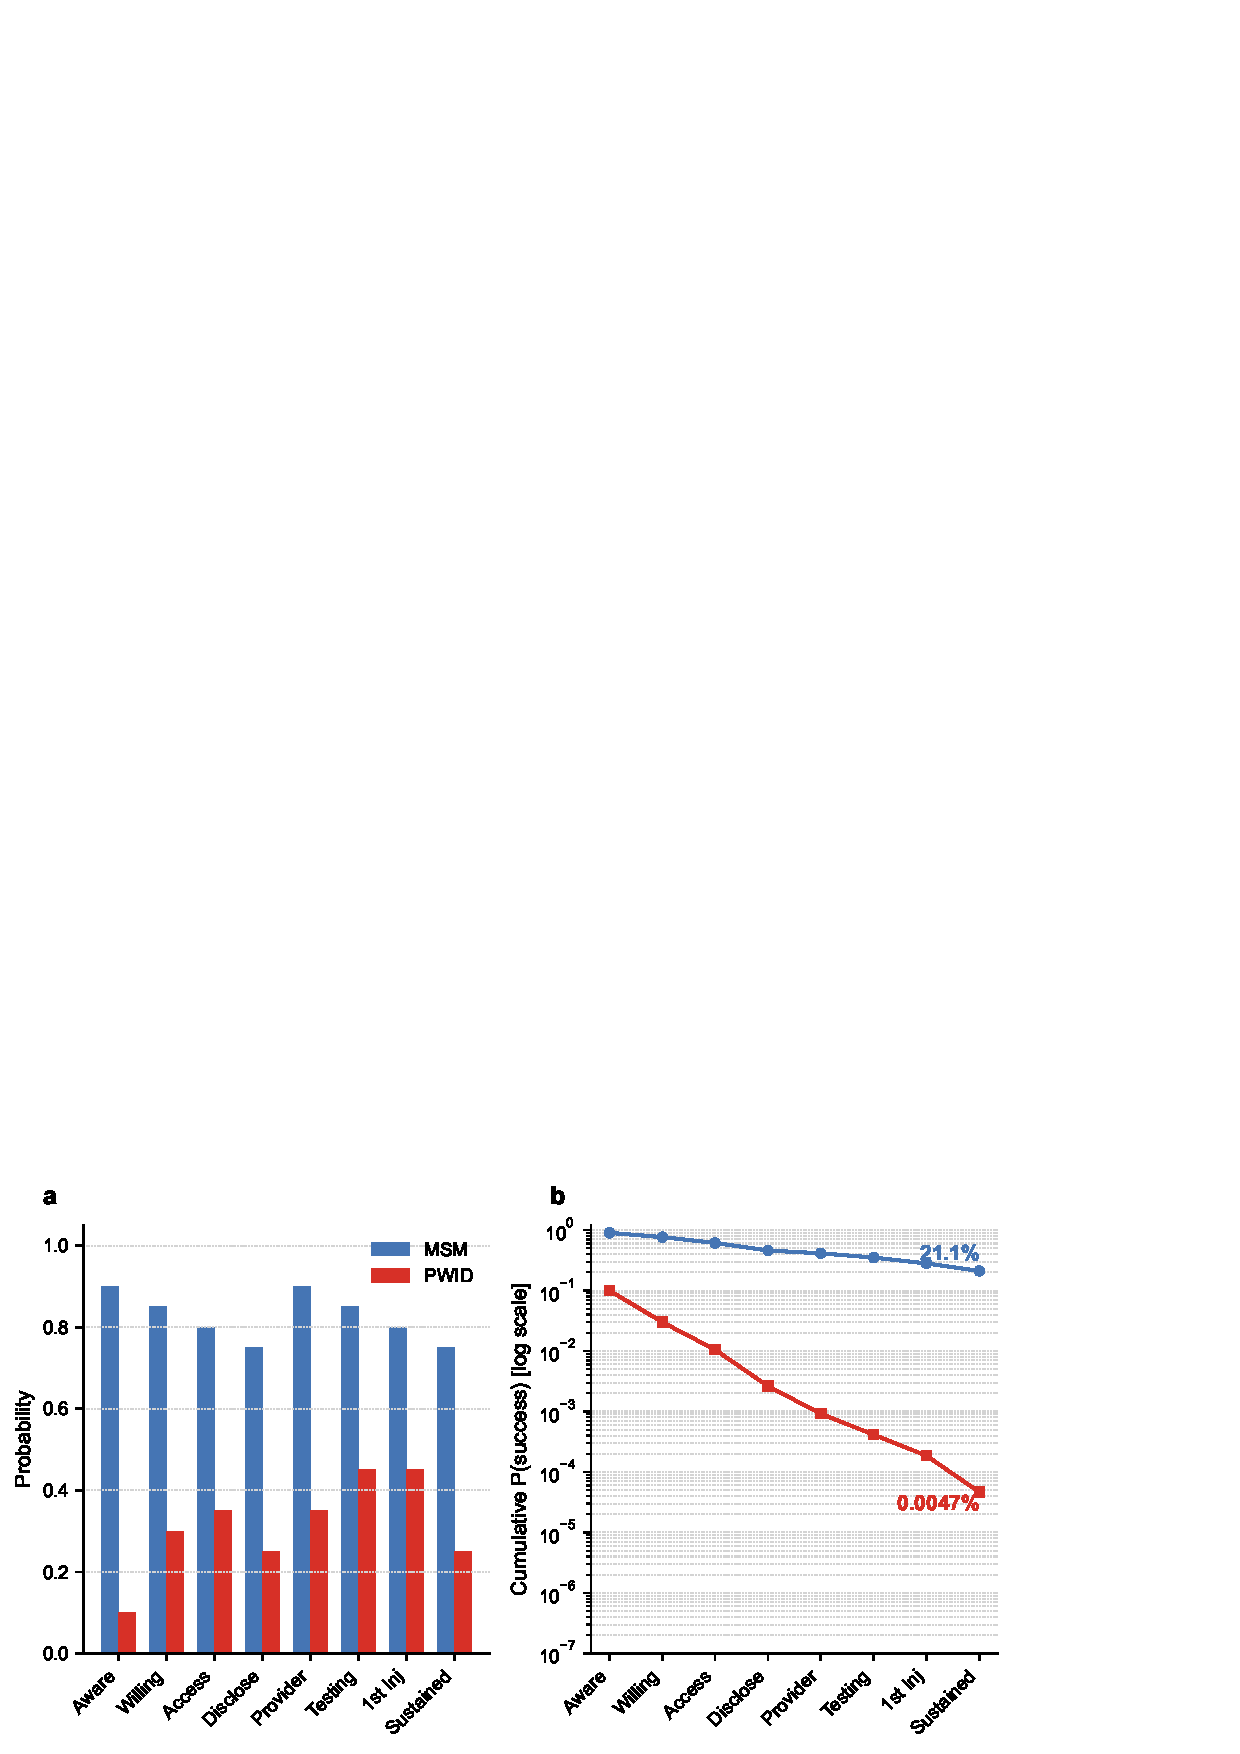
\includegraphics[width=\textwidth]{Fig1_CascadeComparison.png}
\caption{\textbf{LAI-PrEP Cascade Comparison: MSM vs PWID.} Step-wise probabilities showing barrier-adjusted probability of completing each cascade step, demonstrating the dramatic disparity between MSM (cascade completion 21.1\%) and PWID (cascade completion 0.0047\%). Under current policy, 90\% of PWID fail at the awareness step.}
\label{fig:cascade}
\end{figure}

\subsection{Three-Layer Barrier Decomposition}

Barrier decomposition attributed failures as follows: Layer 1 (Pathogen Biology) 0.0\%, Layer 2 (HIV Testing) 6.8\%, and Layer 3 (Architectural Failures) 93.2\% (Figure 2). Within architectural failures, policy barriers (criminalization and incarceration) contributed 38.4\%, infrastructure barriers (MSM-centric design) 21.9\%, stigma barriers (healthcare discrimination) 20.5\%, machine learning barriers (algorithmic deprioritization) 8.2\%, and research exclusion barriers 4.1\%.
These findings are consistent with extensive evidence demonstrating incarceration as a key structural driver of HIV transmission risk, treatment interruption, and prevention failure among PWID.\cite{altice_perfect_storm_2016}

Notably, pathogen biology contributed 0.0\% to prevention failure because cascade attrition was so severe that very few individuals reached the point where pathogen dynamics became relevant. The irreversibility of HIV integration within hours remains fundamental to the requirement for \Rzero{}=0, but this biological constraint is never tested when 90\% fail at awareness.

\begin{figure}[ht]
\centering
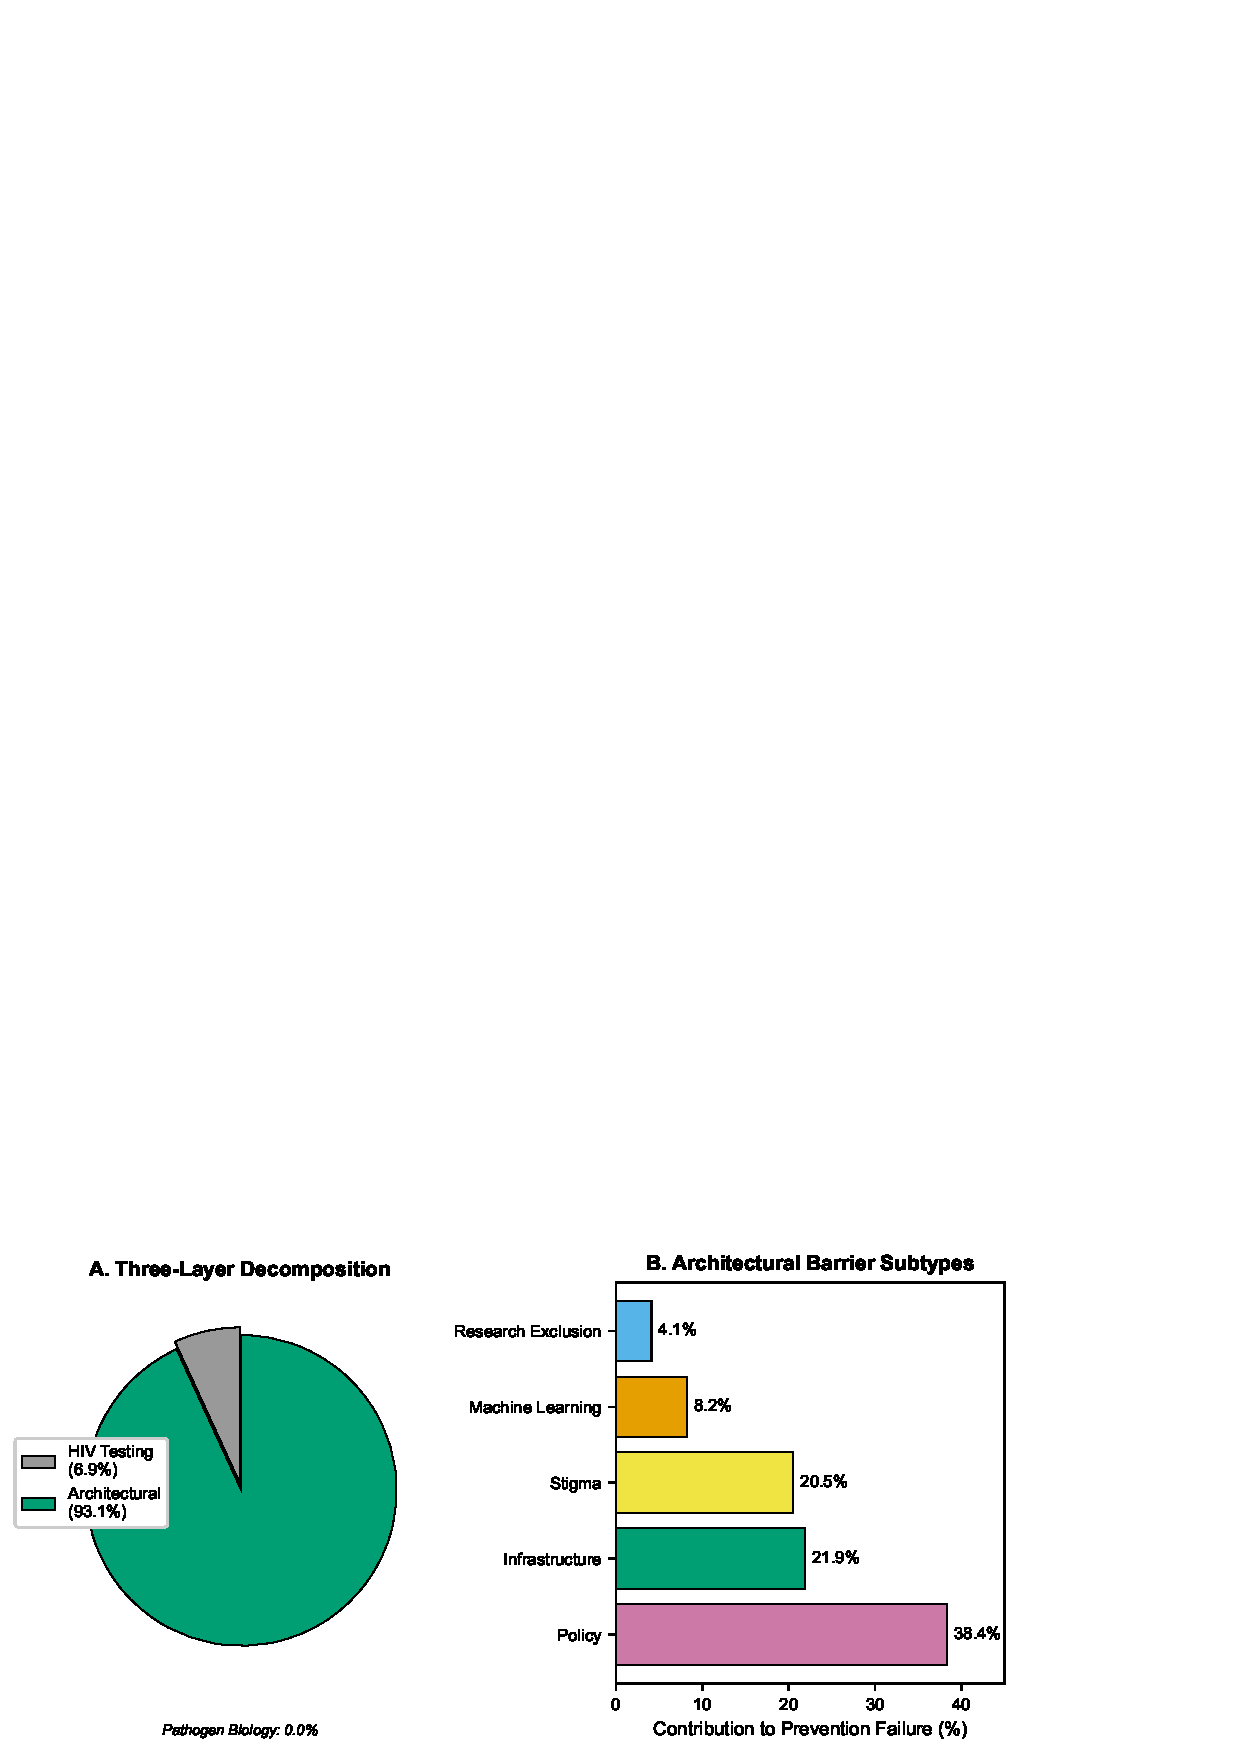
\includegraphics[width=\textwidth]{Fig2_BarrierDecomposition.png}
\caption{\textbf{Three-Layer Barrier Decomposition.} Distribution of prevention failure across three layers: Pathogen Biology (0.0\%), HIV Testing (6.8\%), and Architectural Failures (93.2\%). Within architectural failures: Policy (38.4\%), Infrastructure (21.9\%), Stigma (20.5\%), Machine Learning (8.2\%), and Research Exclusion (4.1\%).}
\label{fig:barriers}
\end{figure}


\subsection{Policy Scenario Analysis}

Table 1 presents P(\Rzero{}=0) across eight policy scenarios. Decriminalization alone increased P(\Rzero{}=0) from 0.00\% to 0.14\% (95\% CI: 0.12--0.17). Adding stigma reduction achieved 0.44\% (95\% CI: 0.40--0.48). SSP-integrated delivery with peer navigation reached 5.03\% (95\% CI: 4.89--5.16). Full harm reduction (SSP + OAT + housing + employment) achieved 9.42\% (95\% CI: 9.24--9.60). Incorporating PURPOSE-4 trial data (if PWID were included) increased this to 11.86\% (95\% CI: 11.66--12.06). Full harm reduction with algorithmic debiasing reached 18.62\% (95\% CI: 18.38--18.86). Theoretical maximum (all barriers removed) achieved 19.92\% (95\% CI: 19.67--20.17).

\begin{figure}[ht]
\centering
\includegraphics[width=\textwidth]{Fig3_PolicyScenarios.png}
\caption{\textbf{Policy Scenario Analysis.} P(\Rzero{}=0) across eight policy scenarios ranging from Current Policy (0.00\%) to Theoretical Maximum (19.92\%), with MSM comparison (16.30\%) shown for reference. SSP-integrated delivery achieves 5.03\%; full harm reduction achieves 9.42\%; algorithmic debiasing adds 9.20 percentage points.}
\label{fig:policy}
\end{figure}

\subsection{MSM vs PWID Disparity}

The MSM population receiving identical LAI-PrEP intervention achieved P(\Rzero{}=0) of 16.30\% compared to 0.00\% for PWID---an extreme disparity spanning several orders of magnitude. This difference emerged entirely from structural factors: MSM cascade step probabilities ranged from 75--95\% compared to 10--45\% for PWID. MSM incarceration survival over 5 years was 77.4\% compared to 16.8\% for PWID. The 120-fold disparity in signal-to-noise ratio (SNR) for machine learning training data (MSM: 9,180 publications; PWID: 76.4) contributed to algorithmic deprioritization that compounds other barriers (Figure 5).

\begin{figure}[ht]
\centering
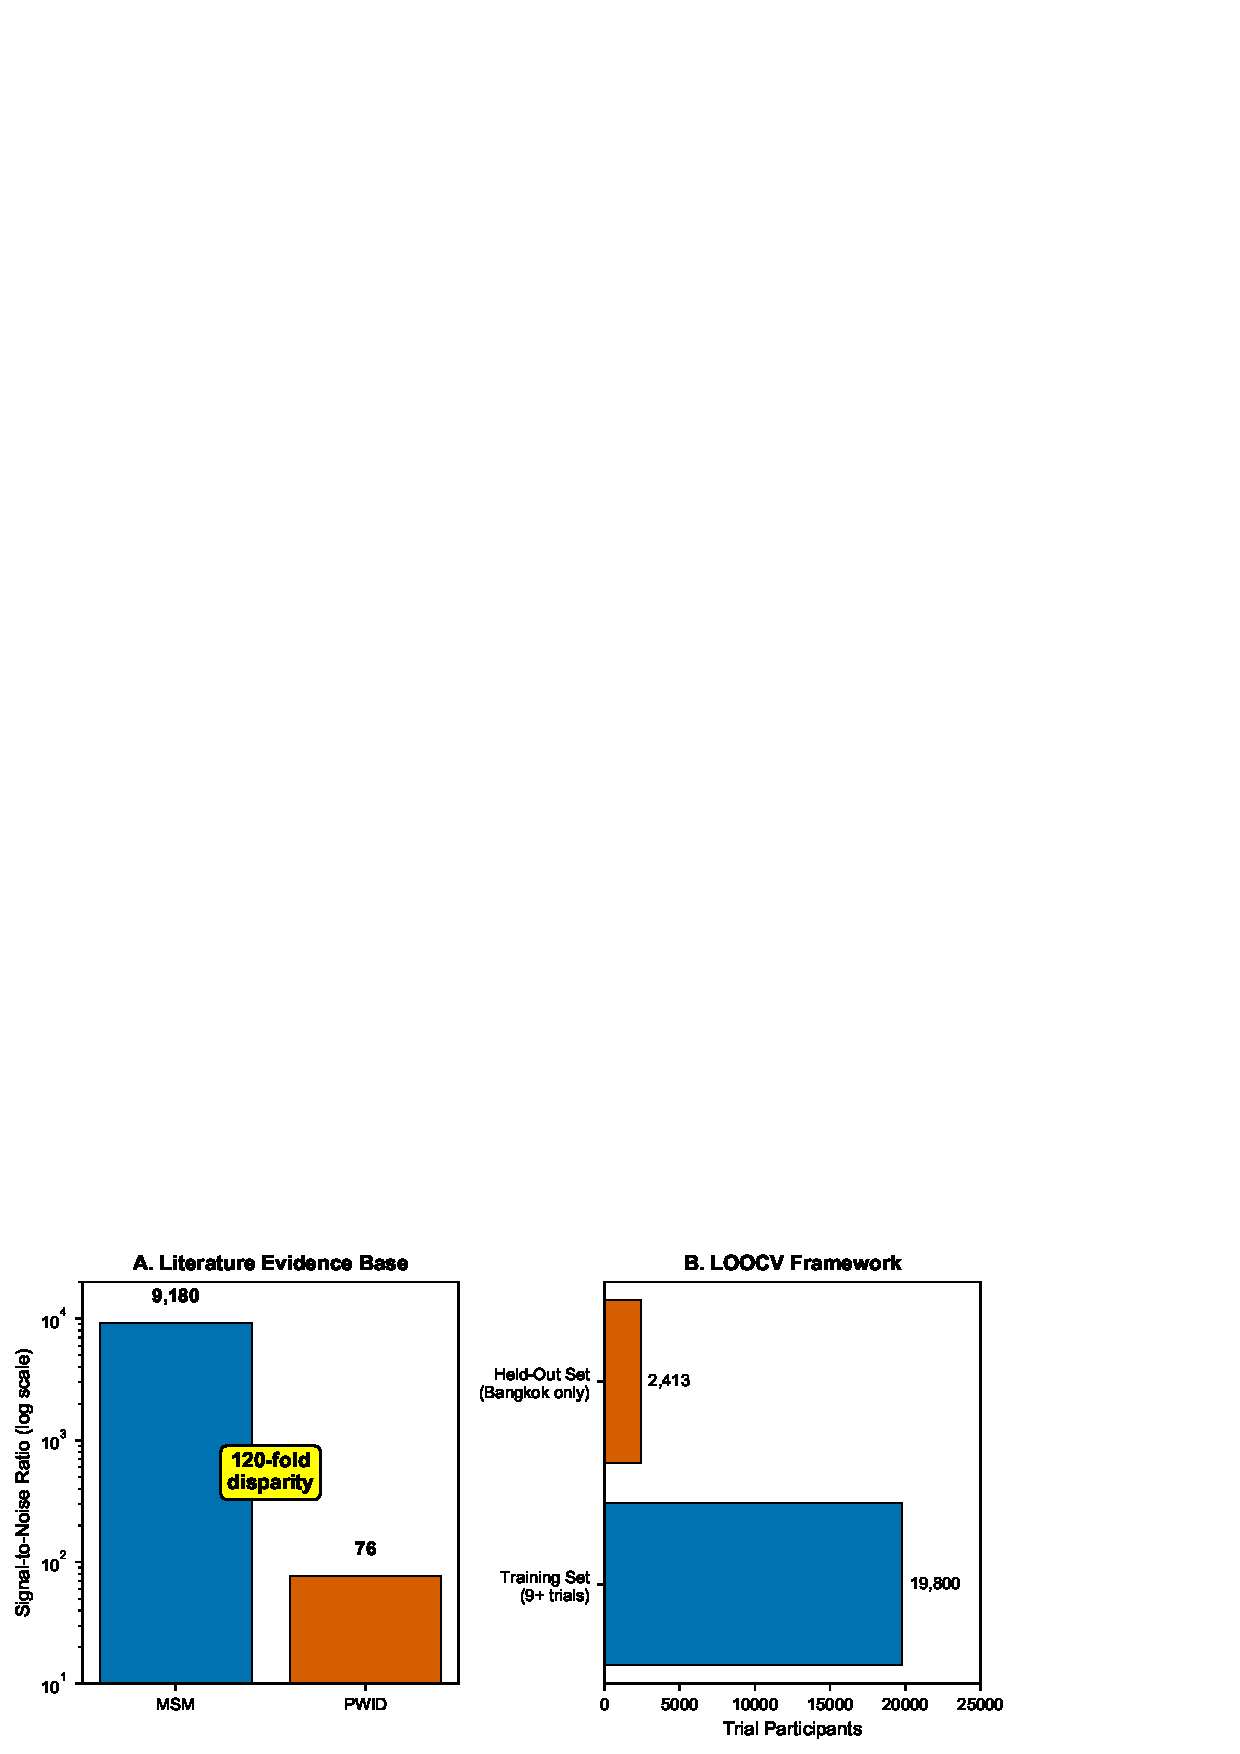
\includegraphics[width=\textwidth]{Fig5_SNR_LOOCV.png}
\caption{\textbf{Signal-to-Noise Ratio Disparity and LOOCV Framework.} Comparison of literature volume supporting machine learning algorithms: MSM (9,180 publications) vs PWID (76.4 publications, estimated)---a 120-fold disparity. The LOOCV framework shows systematic exclusion of PWID from HIV prevention trial evidence base, with PWID functioning as the ``held-out test population'' that was never validated.}
\label{fig:snr}
\end{figure}

\subsection{Stochastic Avoidance Failure Prediction}

The stochastic avoidance model predicted 63.3\% probability of major outbreak within 5 years under current conditions (Figure 4). Median time to outbreak was 4.0 years. Cumulative probability reached 87.6\% by 10 years. Network density trajectory showed progression from 0.895 (2024) toward the critical threshold, driven by methamphetamine prevalence growth.

Regional variation was substantial (Table 2): Pacific Northwest (baseline methamphetamine 35\%) showed 88\% 5-year outbreak probability with median 1.0 year; Appalachia (25\% baseline, 4\%/year growth) showed 78\% with median 2.0 years; Northeast Urban (12\% baseline, 5\%/year growth) showed 64\% with median 3.0 years; National Average showed 59\% with median 4.0 years.

\begin{figure}[ht]
\centering
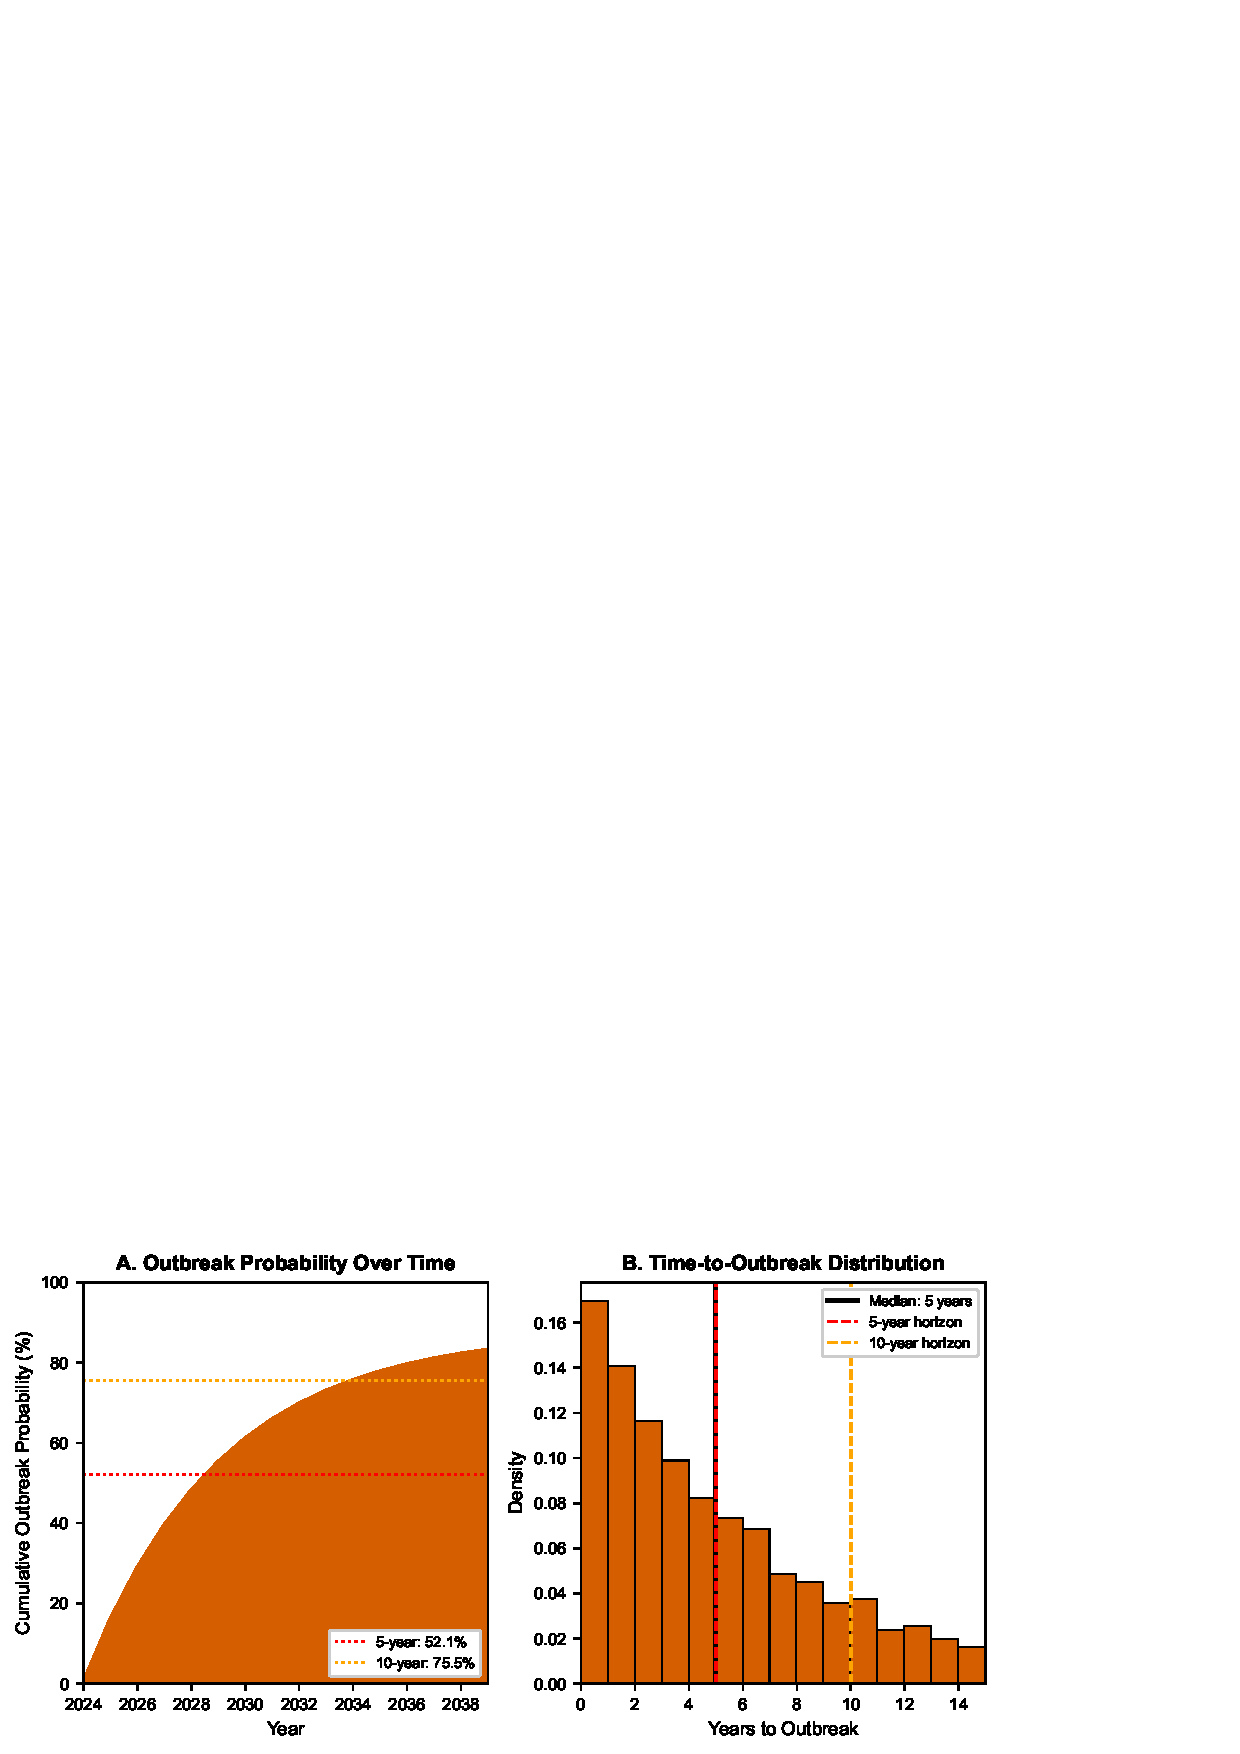
\includegraphics[width=\textwidth]{Fig4_StochasticAvoidance.png}
\caption{\textbf{Stochastic Avoidance Failure Prediction.} Cumulative outbreak probability over time with 90\% confidence interval, showing 63.3\% probability by 5 years and 87.6\% by 10 years. Time-to-outbreak distribution shows median 4.0 years with 80\% credible interval.}
\label{fig:stochastic}
\end{figure}

\subsection{Sensitivity Analysis}

Probabilistic sensitivity analysis confirmed robustness: observed P(\Rzero{}=0) below the resolution of the simulation (95\% CI bounded at zero). Tornado analysis identified baseline outbreak probability ($\pm$49.8 percentage points), critical network threshold ($\pm$17.8pp), and methamphetamine network multiplier ($\pm$16.6pp) as most influential parameters. Barrier removal analysis showed that eliminating criminalization alone increased P(\Rzero{}=0) from 0.00\% to 0.23\%; removing all architectural barriers achieved 19.88\%.

% DISCUSSION
\section{Discussion}
This modeling analysis demonstrates that the limited population-level impact of HIV prevention among people who inject drugs is not explained by drug efficacy or individual behaviour but by the structure of prevention systems within which these agents are deployed. Despite assuming near-perfect pharmacological effectiveness, the probability of PWID achieving sustained protection under current policy conditions approached zero. This finding reflects cumulative attrition across an eight-step prevention cascade, where moderate barriers at each stage compound to render effective prevention highly improbable.

A key insight is that biological constraints—such as rapid reservoir establishment following exposure—account for little of the observed prevention failure under real-world conditions. Instead, most individuals fail to reach the point at which biological factors become relevant. Approximately 90\% of PWID were lost at the awareness stage alone, underscoring the dominance of structural and informational barriers early in the cascade. This observation reframes the prevention challenge: improving pharmacology alone is unlikely to produce meaningful population impact without parallel changes to policy and delivery infrastructure.

Comparison with men who have sex with men, who receive identical pharmacological interventions, illustrates the role of structural context. MSM benefit from prevention architectures designed around their inclusion in clinical trials, regulatory approvals, and implementation studies. In contrast, PWID have largely been excluded from these processes. The resulting disparity in sustained protection is therefore not biological but architectural.

Our stochastic avoidance failure model provides further context. Periods of low HIV incidence among PWID can occur through chance interruption of transmission chains rather than systematic prevention. However, this form of protection is inherently unstable. Increasing methamphetamine use—associated with higher injection frequency, network connectivity, and bridging between populations—erodes stochastic protection and accelerates transition toward outbreak conditions. The projected probability of major outbreaks within five years is consistent with recent epidemiological events and suggests that reliance on chance is unlikely to remain viable.

Policy scenario analyses indicate that isolated interventions are insufficient. Decriminalisation alone or incremental improvements in access modestly increase prevention probabilities but remain far below levels required for epidemic control. Even comprehensive harm reduction strategies achieved sustained protection below 25\%, reflecting the multiplicative nature of cascade barriers. These findings align with prior analyses identifying criminalization and incarceration as central mechanisms through which HIV prevention and treatment are systematically undermined among PWID.\cite{altice_perfect_storm_2016,debeck_criminalization_2017} and highlight the necessity of coordinated, multi-level interventions addressing criminalisation, healthcare access, stigma, testing infrastructure, and continuity of care.

This study has limitations. Cascade parameters were derived from heterogeneous sources, and real-world dynamics may vary across regions. Network modelling simplifies complex social structures, and we did not incorporate re-engagement following cascade failure. Nonetheless, extensive sensitivity analyses demonstrated robustness of the central finding: under plausible parameterisations consistent with existing data, sustained prevention for PWID remains unlikely without substantial structural change.

In conclusion, the gap between pharmacological efficacy and population-level effectiveness in HIV prevention for PWID is driven by policy and implementation barriers rather than biological constraints. Without fundamental changes to prevention architecture, highly efficacious agents will continue to yield minimal population impact, and reliance on stochastic avoidance will leave PWID vulnerable to future outbreaks. Addressing this gap requires reframing HIV prevention not solely as a biomedical challenge but as a structural and policy imperative.

\section{Conclusions}

HIV prevention outcomes among people who inject drugs are shaped primarily by policy and implementation context rather than pharmacological limitations. Under current conditions, the probability of achieving sustained HIV protection for PWID approaches zero despite the availability of highly efficacious prevention agents. In contrast, the same pharmacological interventions achieve substantially higher population-level effectiveness in settings where prevention architectures were designed to support access and continuity.

Current prevention strategies for PWID rely heavily on stochastic avoidance, a time-limited and unstable mechanism that is increasingly undermined by methamphetamine-driven network densification. Modelling results indicate that, without substantial structural change, the likelihood of future HIV outbreaks remains high.

Achieving meaningful epidemic control will require coordinated reforms addressing criminalisation, healthcare access, stigma, prevention infrastructure, research inclusion, and continuity of care. Without such changes, improvements in pharmacological efficacy alone are unlikely to translate into population-level prevention gains for PWID.

\bibliographystyle{elsarticle-num}
\bibliography{unified_lancet_hiv_2025_acd}

\section*{Data Sharing}

All model code, simulation outputs, and analysis scripts are available at \url{https://github.com/Nyx-Dynamics/hiv-prevention-master}. All model inputs derive from published literature or synthetic populations requiring no individual-level data privacy protections.

\section*{Declaration of Interests}

The author declares no competing interests.

\section*{Acknowledgments}

\textbf*{Communities:}
The author thanks the HIV prevention research community whose published work provided model parameters, and the PWID community advocates whose testimony informed barrier characterization.

\textbf*{Non-author Intellectual Contributions:}
The author acknowledges the use of artificial intelligence tools, including Anthropic Claude and OpenAI ChatGPT, to support literature synthesis, code development, and manuscript drafting. These tools were used as assistive technologies only. The author retains full responsibility for study design, data analysis, interpretation of results, and all conclusions presented.  Computational analyses were conducted using Python with open-source packages including NumPy, Pandas, SciPy, Matplotlib, and Seaborn. Code development was performed in JetBrains PyCharm. Reference management was supported using Zotero, and manuscript preparation was conducted using the Overleaf \LaTeX\ platform.

\section*{Author Contributions}
ACD conceived the study, developed the theoretical framework, conducted the literature synthesis, built the computational models, performed all analyses, and wrote the manuscript.

\end{document}


